\subsection{Progettazione di dettaglio e codifica}
\label{progettazione_di_dettaglio}
\textbf{Durata:} dal 2021\_03\_09 al 2021\_04\_02 \\
Il periodo inizia appena concluso il precedente e termina con la \glo{\textbf{RQ}}.
Le precondizioni sono:
\begin{itemize}
    \item Le postcondizioni del periodo precedente sono state soddisfatte.
\end{itemize}
Le postcondizioni sono:
\begin{itemize}
    \item Aggiornamento e correzione dei documenti già prodotti;
    \item Realizzazione dei diagrammi delle classi e delle attività;
    \item Completamento codifica e relativa verifica;
    \item Redazione \textbf{manuale utente} e \textbf{manuale sviluppatore};
    \item Consegna dei documenti richiesti in entrata alla \textbf{RQ};
    \item Ultimata preparazione della presentazione da esporre in sede di revisione.
\end{itemize}
È composto da nuovi incrementi e nuove attività:
\begin{itemize}
    \item \textbf{Incremento e verifica dei documenti (dal 2021\_03\_09 al 2021\_03\_26):} i documenti già prodotti vengono migliorati e aggiornati se necessario ({\NdP}, {\PdP}, {\Glossario}, {\PdQ}, {\AdR});
    \item \textbf{Incremento e verifica delle attività (dal 2021\_03\_09 al 2021\_03\_17)}: viene migliorata l'attività di \glo{TB}, ampliando lo studio delle tecnologie mancanti e progettando ad alto livello come realizzare il prodotto finale;
    \item \textbf{Product Baseline (dal 2021\_03\_09 al 2021\_03\_17):} segue la Technology Baseline e vengono discussi:
        \begin{itemize}
            \item \textbf{Design pattern}: vengono individuati e discussi in modo da capire quali siano necessari e come riuscire a integrarli al meglio nel progetto;
            \item \textbf{Diagrammi classi}: dopo un'attenta riflessione sul codice vengono realizzati i diagrammi delle classi;
            \item \textbf{Diagrammi attività}: dopo un'attenta riflessione sul codice vengono realizzati i diagrammi delle attività. 
        \end{itemize} 
    \item \textbf{Specifica tecnica(dal 2021\_03\_18 al 2021\_03\_26):} viene realizzato un documento contenente tutte le caratteristiche del prodotto e le motivazioni che hanno portato alla loro scelta;
    \item \textbf{Codifica (dal 2021\_03\_18 al 2021\_04\_06):} viene scritto il codice con relativa verifica. Questa attività, dato il modello di sviluppo scelto, verrà suddivisa in 3 incrementi che verranno definiti dopo aver preparato il Proof of Concept così da avere una maggiore conoscenza sul lavoro effettivo da svolgere e poter progettare al meglio i vari incrementi;
    \item \textbf{Manuale utente e manutentore(dal 2021\_03\_24 al 2021\_04\_06):} documenti redatti rispettivamente per indicare le istruzioni d'uso specifiche per l'utente e per supportare eventuali sviluppatori attraverso la descrizione dell'architettura del sistema.
\end{itemize}
\subsubsection{Incrementi del periodo}\label{IncrementiPDettaglio}
\begin{table}[H]
	\begin{center}
		\begin{tabular}{ |C{3cm} C{6cm} C{7cm}| }
			\rowcolor{darkblue} 
			\textcolor{white}{\textbf{Incremento}} & \textcolor{white}{\textbf{Obiettivi}} & \textcolor{white}{\textbf{Requisiti}} \\ \hline
			I dal 2021\_03\_09 al 2021\_03\_17& Miglioramento della documentazione già prodotta, ampliamento dello studio delle tecnologie, studio di \glo{design pattern}, diagrammi delle classi e delle attività.  & - \\ \hline
			II dal 2021\_03\_18 al 2021\_03\_26 	& Correzione dei documenti post \glo{RP}, redazione dell'allegato tecnico, inizio sviluppo del codice e redazione manuali. &  
			RFO1\_1 - RFO6\_1.1.5, RFO7\_2 \newline
			RFO8\_3, RFO10\_4, RFO11\_5 \newline
			RFO59, RFO60 \newline
			RFO61\_23 - RFO64\_23.3, RFO65\_24 \newline
			RF067, RFO68\_25 - RFO72\_25.4 \newline
			RFO73\_26, RFO74, RFO75, RFO11\_5, \newline 
			RFO12\_ 6 - RFO15\_ 6.3, RFO16 \newline RFO17, RFO18, RFO19\_7\newline RFO20\_8, RFO21\_9, RFO22\_10 \newline RFO23, RFO26, RFO27 \newline RFO29\_12, RFO66, RFO76 \newline RFO77, RFO78, RFO80 \\ \hline
			III dal 2021\_03\_27 al 2021\_04\_01 	& Continuazione nello sviluppo del codice e nella redazione manuali, preparazione alla \glo{PB}. & RFO81\_27 - RFO88\_27.7 \newline
			RFO89, RFO90\_28 - RFO97\_28.7 \newline
			RFO98\_29, RFO99\_30, RFO100\_31 \newline
			RFO101\_32, RFO102\_33 \newline
			RFO103\_34 - RFO107\_34.4, RFO108 \newline
			RFO109\_35 - RFO110\_35.1\newline
			RFO111\_36 - RFO112\_36.1, RFO113\_37 \newline RFO114\_38, RFO115, RFO25 \newline RFO30, RFO31\_13, RFO32\_13 \newline RFO33\_14, RFO34\_15, RFO35\newline  RFO36, RFO37\_16, RFO40\_16.1 \\ \hline
			III dal 2021\_04\_01 al 2021\_04\_06 	& 
			Conclusione della redazione del codice e dei manuali, preparazione alla \glo{RQ}. & RFO24, RFO38, RFO39\newline RFO40\_16.1,
			RFO41\_17 - RFO45\_17.1.4\newline
			RFO46\_18 - RFO50\_18.4, RFO51\_19 \newline
			RFO52, RFO53\_20, RFO54\_20 \newline
			RFO55\_21, RFO56\_22 - RFO58\_22.2 \newline
			RFO79, RFO116\_39, RFO117\_39 \newline RFO118\_40, RFO119, RFO120\_41 \newline
			RFO121\_42, RFO122\_43 - RFO126\_43.2.2 \\ \hline
		\end{tabular}
		\caption{Tracciamento incrementi-obiettivi}
	\end{center}
\end{table}

\newpage
\subsubsection{Diagramma di Gantt: Progettazione di dettaglio e codifica} \label{GanttPDettaglio}
\begin{figure}[ht]
    \centering
    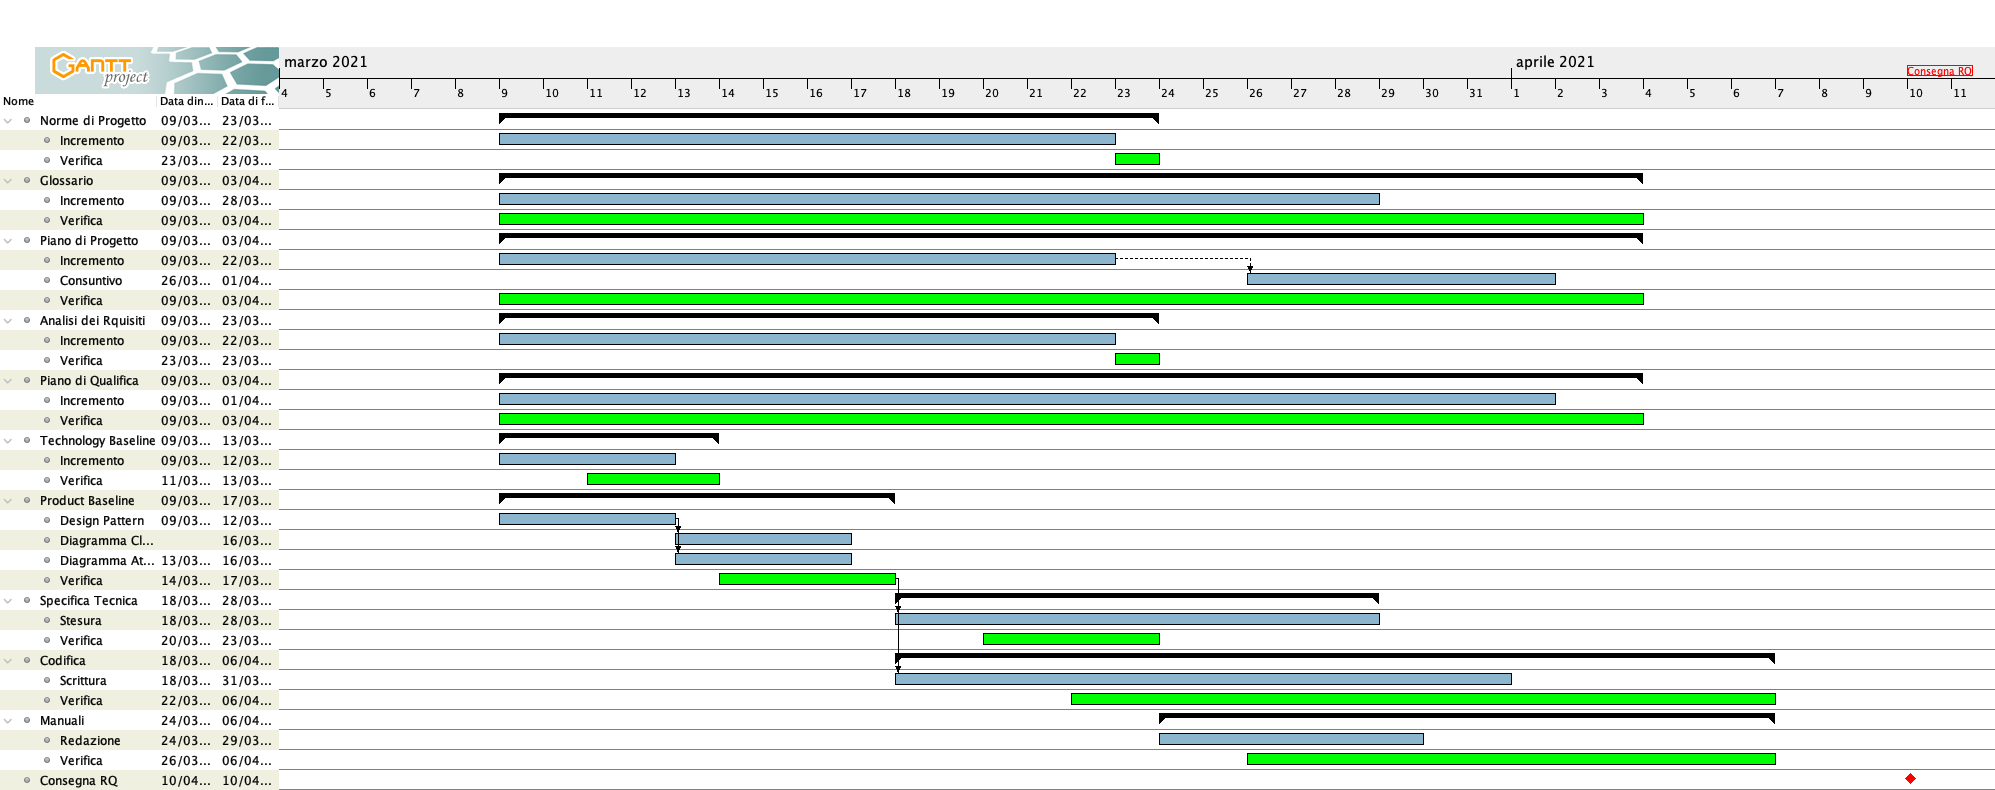
\includegraphics[width=\textwidth]{Immagini/GanttProgettazioneDiDettaglioECodifica}
    \caption{Diagramma di Gantt dell'attività di progettazione di dettaglio e codifica}
\end{figure}